%%%%%%%%%%%%%%%%%%%%%%%%%%%%%%%%%%%%%%%%%%%%%%%%%%%%%%%%%%%%%%%%%%%%%%%%%%%%%%%%
% Memoria para trabajos y entregas de laboratorio de la Escuela Superior de    %
% Informática (ESI) de Ciudad Real, UCLM.                                      %
%   Versión: Octubre - 2018                                                    %
%   Desarrollada por José Ángel Martín Baos                                    %
%                                                                              %
% Recursos:			                                                           %
%   - Contenidos del curso “LaTeX esencial para preparación de Trabajo Fin de  %
%     Grado, Tesis y otros documentos académicos” impartido por el profesor    %
%     Jesús Salido.                                                            %
%                                                                              %
% Disponible en: https://github.com/JoseAngelMartinB/PlantillaTrabajosLaTeX    %
%%%%%%%%%%%%%%%%%%%%%%%%%%%%%%%%%%%%%%%%%%%%%%%%%%%%%%%%%%%%%%%%%%%%%%%%%%%%%%%%

\documentclass[11pt]{article}

% PAQUETES USADOS:
\usepackage{natbib}
\usepackage{url}
\usepackage[utf8]{inputenc} % Codificación (Permite carácteres españoles)
\usepackage{amsmath}
\usepackage{graphicx}
\graphicspath{{images/}} % Carpeta en la cual se van a buscar las imagenes
\usepackage{subfigure}	% Permite la Inclusión de subfiguras
%\usepackage{parskip} % Suprime la identación de los parrafos.
\setlength{\parskip}{3mm} % Longitud del espaciado entre parrafos
\usepackage[hidelinks]{hyperref} % Referencias (links)
\usepackage{fancyhdr}
\usepackage{vmargin}
\usepackage{paralist} % Permite un mayor control sobre las listas
\usepackage{textcomp,marvosym,pifont} % Generación de símbolos especiales
\usepackage[usenames,dvipsnames,svgnames,x11names,table]{xcolor}

% CONFIGURACIÓN DE LA PÁGINA:
\setpapersize{A4} % Formato del papel - A4
\setmarginsrb{3 cm}{2.5 cm}{3 cm}{2.5 cm}{1 cm}{1.5 cm}{1 cm}{1.5 cm} % Margenes

% Complemento para insertar código en la memoria:
%   Basado en 'Listados de código cómodos y resultones con listings'
%   de David Villa en http://crysol.org/es/node/909
\usepackage{color}
\definecolor{gray97}{gray}{.97}
\definecolor{gray75}{gray}{.75}
\definecolor{gray45}{gray}{.45}
\usepackage{listings}
\lstset{ frame=Ltb,
	framerule=0pt,
	aboveskip=0.5cm,
	framextopmargin=3pt,
	framexbottommargin=3pt,
	framexleftmargin=0.4cm,
	framesep=0pt,
	rulesep=.4pt,
	backgroundcolor=\color{gray97},
	rulesepcolor=\color{black},
	texcl=true,
	%
	stringstyle=\ttfamily,
	showstringspaces = false,
	basicstyle=\small\ttfamily,
	commentstyle=\color{gray45},
	keywordstyle=\bfseries,
	%
	numbers=left,
	numbersep=15pt,
	numberstyle=\tiny,
	numberfirstline = false,
	breaklines=true,
}
% Minimizar fragmentado de listados
\lstnewenvironment{listing}[1][]
{\lstset{#1}\pagebreak[0]}{\pagebreak[0]}

\lstdefinestyle{consola}
{basicstyle=\scriptsize\bf\ttfamily,
	backgroundcolor=\color{gray75},
}

\lstdefinestyle{C}
{language=C,
}

%OTROS PAQUETES:
\usepackage{float} % Permite usar H en las figuras, de manera que se coloquen en la posición exacta en la que están en el código.

% Añade un comando para crear indicaciones de pulsación de teclas
\usepackage{tikz} % Paquete especializado en gráficos
\usetikzlibrary{shadows} % Necesario para poder crear nuevo comando de indicación de pulsación de tecla.
\newcommand*\tecla[1]{%
	\tikz[baseline=(key.base)]
	\node[%
	draw,
	fill=white,
	drop shadow={shadow xshift=0.25ex,shadow yshift=-0.25ex,fill=black,opacity=0.75},
	rectangle,
	rounded corners=2pt,
	inner sep=1pt,
	line width=0.5pt,
	font=\scriptsize\sffamily
	](key) {#1\strut}
	;
}

\newif\ifspanish % Condicional que permite seleccionar el lenguage.
\newif\ifmultipleauthors % Condicional que permite multiples autores
\spanishtrue
\multipleauthorsfalse


%%%%%%%%%%%%%%%%%%%%%%%%%%%%%%%%%%%%%%%%%%%%%%%%%%%%%%%%%%%%%%%%%%%%%%%%%%%%%%%%
%%%%%%%%%				Principales variables del documento			   %%%%%%%%%

\title{Práctica 1: Red Toroide e Hipercubo}							% Titulo
\author{David Camuñas Sánchez}							% Autor

\date{\today}											% Fecha
\newcommand{\subject}{Diseño de Infraestructuras de Red}						% Asignatura
\newcommand{\course}{Grado en Ingeniería Informática}	% Curso
%\newcommand{\course}{Máster Universitario en Ingeniería Informática}	% Curso
\newcommand{\courseyear}{2019 - 2020} 					% Curso académico
%\spanishfalse	    	% Descomentar esta línea si el trabajo está en inglés
%\multipleauthorstrue   % Descomentar esta línea si hay varios autores

%%%%%%%%%%%%%%%%%%%%%%%%%%%%%%%%%%%%%%%%%%%%%%%%%%%%%%%%%%%%%%%%%%%%%%%%%%%%%%%%

\ifspanish
	\usepackage[spanish]{babel} % Paquete de español
	\newcommand{\dateText}{Fecha:}
	\renewcommand{\lstlistingname}{Listado} % Renombrar listados para que aparezcan en español.
	% Algoritmos
	\usepackage[ruled,vlined,spanish]{algorithm2e} % Permite pseudocódigos. NECESARIO INSTALAR texlive-science (sudo apt-get install texlive-science)
\else
	\usepackage[english]{babel} % Paquete de inglés
	\newcommand{\dateText}{Date:}
	% Algoritmos
	\usepackage[ruled,vlined,english]{algorithm2e}
\fi

\makeatletter
\let\thetitle\@title
\let\theauthor\@author
\let\thedate\@date
\makeatother

% Formato de página:
\pagestyle{fancy}		% Formato por defecto - Recomendado
%\pagestyle{headings} 	% Formato para libros
\fancyhf{}
\ifmultipleauthors
	\chead{\thetitle}
\else
	\rhead{\theauthor}
	\lhead{\thetitle}
\fi
\cfoot{\thepage}

\begin{document}

%%%%%%%%%%%%%%%%%%%%%%%%%%%%%%%%%%%%%%%%%%%%%%%%%%%%%%%%%%%%%%%%%%%%%%%%%%%%%%%%
%%%%%%%%							Portada							   %%%%%%%%%

\begin{titlepage}
	\centering
	\begin{minipage}[t]{\textwidth}
		\raisebox{-0.5\height}{
\includegraphics[scale = 0.8]{UCLM_Logo.pdf}} 	% Logo de la universidad
		\hspace{\fill}
	\end{minipage}
	\\[2.25 cm]
    \textsc{\LARGE Universidad de Castilla-La Mancha}\\[1 cm]	% Nombre de la universidad
    \textsc{\LARGE Escuela Superior de Informática}\\[2.0 cm]
	\textsc{\Large \subject}\\[0.5 cm]				% Asignatura
	\textsc{\large \course \\ \courseyear}\\[2 cm]				% Curso
	\rule{\linewidth}{0.2 mm} \\[0.4 cm]
	{ \huge \bfseries \thetitle}\\
	\rule{\linewidth}{0.2 mm} \\[2.5 cm]

	\vspace*{\fill}
	\begin{minipage}{0.4\textwidth}
		\begin{flushleft} \large
			\ifspanish
				\ifmultipleauthors
					\emph{Autores:}\\
				\else
					\emph{Autor:}\\
				\fi
			\else
				\ifmultipleauthors
					\emph{Authors:}\\
				\else
					\emph{Author:}\\
				\fi
			\fi
			\theauthor
			\end{flushleft}
			\end{minipage}~
			\begin{minipage}{0.4\textwidth}
			\begin{flushright} \large
			\emph{\dateText} \\
			\thedate
		\end{flushright}
	\end{minipage}\\[2.25 cm]


\end{titlepage}

%%%%%%%%%%%%%%%%%%%%%%%%%%%%%%%%%%%%%%%%%%%%%%%%%%%%%%%%%%%%%%%%%%%%%%%%%%%%%%%%
%%%%%%%%%						   	Índice					      	   %%%%%%%%%

\tableofcontents
\pagebreak


%%%%%%%%%%%%%%%%%%%%%%%%%%%%%%%%%%%%%%%%%%%%%%%%%%%%%%%%%%%%%%%%%%%%%%%%%%%%%%%%
%%%%%%%%%							Documento						   %%%%%%%%%

% Sección: Intruducción
\section{Introducción}
El objetivo de esta primera fase de la práctica es la creación de uno de los tipos de redes de comunicación existente, esta es la \textbf{\textit{red Toroide}} o \textit{de anillo}.

A la hora de dibujar este tipo de red para entender su funcionamiento, se puede mostrar como una matriz. 

Cuya peculiaridad es que son redes cuadradas, de \textit{lado} \textit{\textbf{L}}, donde cada fila o columna de un extremo, conecta con su fila o columna inversa, es decir, los elementos que formarían la última fila de la matriz se conectarían (serían \textit{"vecinos"}) con los elementos de la primera fila de la matriz y asi sucesivamente.

A continuación, se mostrará un ejemplo donde se puede observar la estructura de este tipo de red.

\begin{figure}[h!]
  \centering
  \subfigure[Red toroide en 3D]{
    
\includegraphics[width=70mm]{toroide.png}
  }
  \subfigure[Topología de una red Toroide]{
  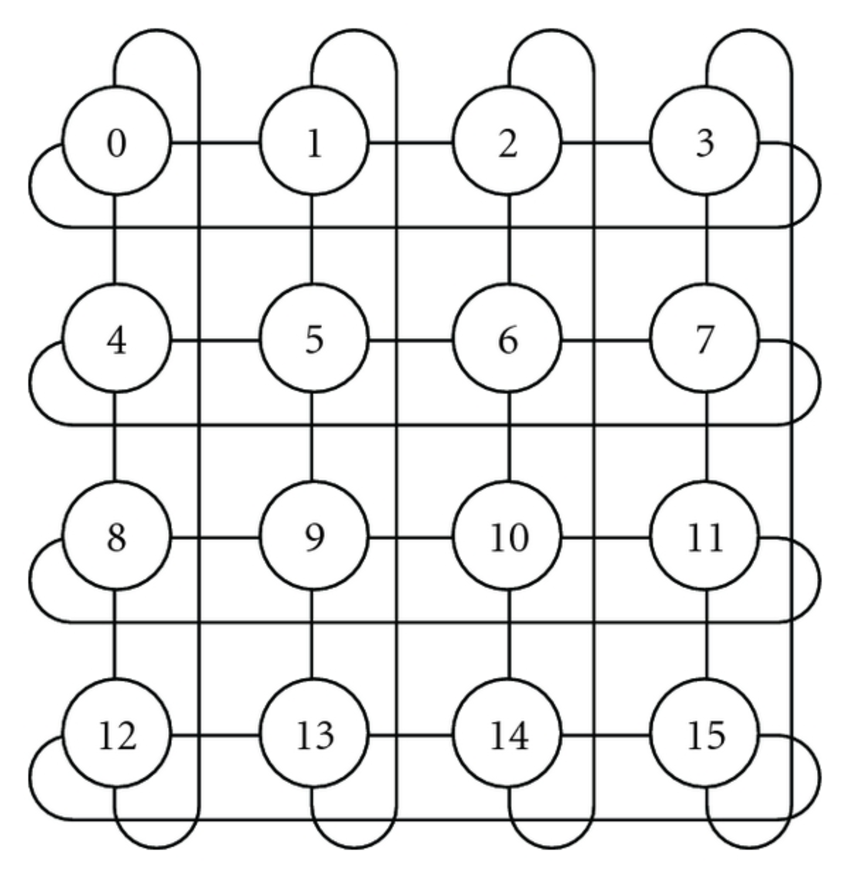
\includegraphics[width=70mm]{toroide-r.png}
  

  }
  \caption{Imágenes Red Toroide}
  \label{fig:toroide}
\end{figure}

\clearpage


\section{Planteamiento de la solución}
Para solucionar el problema, se tiene en cuenta que una \textit{red Toroidal} tiene un valor de \textit{\textbf{lado L}}.
Donde el \textit{número de procesos} \textbf{N} esta determinado por: \textbf{$L^{2}$}

En este caso el valor de \textbf{L} es \textbf{3}, por lo tanto, el valor de \textbf{N} será \textbf{9}, esto quiere decir que este toroide estaŕa formado por 9 procesos (denominados en el código como \textit{ranks}).

El número de lado \textbf{L} del toroide se encuentra definido en \textit{/include/definitions}, como:

\textit{\textbf{define L 3}}

Si se quiere realizar la simulación con un valor de lado distinto, se deberá cambiar el valor de esta constante. Además del número total de procesos a crear, pasado como argumento al comando de ejecución (\textit{mpirun}) en la línea de ordenes. Este valor se puede encontrar en el \textit{Makefile} del proyecto.

Otra constante importante, es la que determina el tamaño del buffer lectura del fichero (en este caso \textit{datos.dat}), debido a que si se quiere leer una gran cantidad de números, y asi crear una gran cantidad de nodos (ranks), se debe de modificar su valor a uno mayor.

\textit{\textbf{define MAX-SIZE 1024}}

\subsection{Tipos de nodos}
En este problema encontramos dos tipos de nodos: el \textbf{\textit{rank o nodo 0}} y los demás \textbf{\textit{nodos}}.

\begin{itemize}
	\item \textbf{Rank 0}: Este nodo corresponde al primer proceso creado. Encargado de la lectura del fichero \textit{\textbf{datos.dat}}, el cual contiene los números que más tarde asignara el mismo a los demás nodos que forman la red toroidal.
	
	A la hora de realizar la asignación de los números a los respectivos nodos restantes (incluyendose el mismo), debe de comprobar que la cantidad de números obtenidos del fichero es igual al tamaño del toroide \textbf{N} (nº de nodos que lo forman) si esta comprobación es exitosa, continuara la ejecución normal del programa.
	
	En caso contrario, a mi elección bien sea por que el tamaño del toroide o la cantidad de los números sea menor o mayor. El \textit{rank 0} cero abortará la ejecución del programa. 
	Tanto si la comprobación es correcta como si no, este difundirá el resultado a los demás nodos. Para ello se ha utilizado la función \textit{Bcast()} de la libreria de \textbf{MPI}.
	
	Una vez asignados los respectivos números a cada nodo, tras calcular el número mínimo de la red toroidal, \textit{rank 0} mostrara dicho número por pantalla, y el programa finalizará.
	
	\item \textbf{Los demás nodos}: Estos tipos de nodos recibirán del \textit{rank 0} la decisión de continuar o no. Si continua la ejecución normal se les asignará un número real, el cual trás obtener cada uno sus respectivos vecinos, se  llevará a cabo el algoritmo para obtener \textbf{el menor número de la red toroidal}.
\end{itemize}



%%%%%%%%%%%%%%%%%%%%%%%%%%%%%%%%%%%%%%%%%%%%%%%%%%%%%%%%%%%%%%%%%%%%%%%%%%%%%%%%
%%%%%%%%% 						BIBLIOGRAFIA 						   %%%%%%%%%
%%%%%%%%%%%%%%%%%%%%%%%%%%%%%%%%%%%%%%%%%%%%%%%%%%%%%%%%%%%%%%%%%%%%%%%%%%%%%%%%
\newpage
\bibliography{biblist}
\bibliographystyle{plain}
%\nocite{*} Permite citar todas las referencias en el archivo .bib

% Añadir la bibliografía al Índice de contenidos
\ifspanish
	\addcontentsline{toc}{section}{Referencias}
\else
	\addcontentsline{toc}{section}{References}
\fi



%%%%%%%%%%%%%%%%%%%%%%%%%%%%%%%%%%%%%%%%%%%%%%%%%%%%%%%%%%%%%%%%%%%%%%%%%%%%%%%%
%%%%%%%%% 					Atribución - ¡No Eliminar!				   %%%%%%%%%
%%%%%%%%%%%%%%%%%%%%%%%%%%%%%%%%%%%%%%%%%%%%%%%%%%%%%%%%%%%%%%%%%%%%%%%%%%%%%%%%
\null\vfill
\begin{center}
\ifspanish
	Este documento ha sido generado con \LaTeX{} utilizando la plantilla\\
	desarrollada por \textsc{José Ángel Martín Baos} y disponible en\\
	\url{https://github.com/JoseAngelMartinB/PlantillaTrabajosLaTeX}
\else
	This document was generated using \LaTeX{} and the template\\
	developed by \textsc{José Ángel Martín Baos} which is available in\\
	\url{https://github.com/JoseAngelMartinB/PlantillaTrabajosLaTeX}
\fi
\end{center}

\end{document}
